\begin{document}

\def\title{Worksheet 2}

\newcommand{\qitem}{\qpart\item}

\renewcommand{\labelenumi}{(\alph{enumi})} % change default enum format to (a)
\renewcommand{\theenumi}{(\alph{enumi})} % fix reference format accordingly.
\renewcommand{\labelenumii}{\roman{enumii}.} % second level labels.
\renewcommand{\theenumii}{\roman{enumii}.}

\maketitle

\vspace{0.5em}

\begin{qunlist}

% {\Large \textbf{Mechanical:}}
\qns{Complex Numbers}

A complex number, $z$, is composed of a real part and imaginary part.
If $z = a + bj$, then $re(z) = a$ (the real portion equals a), and $im(z) = b$ (the imaginary portion equals b).
Complex numbers can be expressed in two ways:

\begin{center}
Rectangular Form: $z = a + bj$ \hspace{1em} Polar Form: $z = re^{j\theta}$
\end{center}

In polar form, $r$ represents the magnitude and $\theta$ represents the angle of the complex number with respect to the origin of the complex plane.
Rectangular form makes adding and subtracting complex numbers easier; whereas, polar form makes multiplying and dividing numbers easier.
Some handy equations to switch between forms include:

\begin{center}
\begin{tabular}{ c c c }
 $tan(\theta) = \frac{b}{a}$ & $r = |z| = \sqrt{a^2 + b^2}$ \\ \\
 $sin(\theta) = \frac{b}{|z|}$ & $cos(\theta) = \frac{a}{|z|}$ \\  \\
\end{tabular}
\end{center}

\begin{enumerate}

\qitem Prove algebraically that $\frac{1}{j} = -j$.

\sol{
The key is to multiply the left-hand side of the equation by $\frac{j}{j}$: \\
$$\frac{1}{j} = \frac{1 * j}{j * j} = \frac{j}{j^2}$$
$$= \frac{j}{-1} = -j$$
}

\end{enumerate}

A complex number, $z = a + bj$ has a complex conjugate, $\overline{z} = a - bj$.
Note that the sum of a complex number and its conjugate is always real, but the difference between a complex number and its conjugate is always imaginary.

\begin{enumerate}[resume]

\qitem Use a polar graph to show that the sum of any complex number and its conjugate is always real.

\sol{

}

\qitem Recall that Euler's Formula states that $e^{j\theta} = cos(\theta) + jsin(\theta)$.
Using Euler's identity, show that $cos(\theta) = \frac{1}{2}(e^{j\theta} + e^{-j\theta})$.

\sol{

  $$e^{j\theta} = cos(\theta) + jsin(\theta)$$

  Note that $e^{j\theta}$ has the complex conjugate $e^{-j\theta}$, which means:

  $$e^{-j\theta} = cos(\theta) - jsin(\theta)$$
  $$e^{j\theta} +  e^{-j\theta} = cos(\theta) + jsin(\theta) + cos(\theta) - jsin(theta)$$
  $$e^{j\theta} +  e^{-j\theta} = 2cos(\theta)$$
  $$cos(\theta) = \frac{1}{2}(e^{j\theta} +  e^{-j\theta})$$

}

\end{enumerate}

\newpage
% Source: Siddharth Iyer, Spring 2018 Discussion 3B
% Updated: Justin Yu (justinvyu@berkeley.edu)

\qns{Introduction to Phasor Domain and Impedance}

\meta{
Tell students that there's a $\frac{1}{2}$ in this semester's definition of the phasor.
Let them know that they may find definitions of phasors (like other semesters of 16b) where the $\frac{1}{2}$ is omitted.
Be sure to tell them that this doesn't change anything at all since we end up factoring it out later anyways.
}

We consider sinusoidal voltages and currents of the general form:

\vspace{-15px}
\begin{align*}
v(t) = V_0 \cos(\omega t + \phi_v) \\
i(t) = I_0 \cos(\omega t + \phi_i)
\end{align*}
\vspace{-15px}

\renewcommand{\arraystretch}{1.5}

where:

\begin{enumerate}
\item
    $V_0$ is the voltage \textbf{magnitude/amplitude} and is the highest value of voltage $v(t)$ will attain at any time. Similarly, $I_0$ is the current
    amplitude.
\item
    $\omega$ is the \textbf{frequency} of oscillation, corresponding to the sinusoid's period $T = \frac{2\pi}{\omega}$.
\item
    $\phi_v$ and $\phi_i$ are the \textbf{phase} terms of the voltage and current respectively. These capture a delay, or shift, in time.
\end{enumerate}

We know from Euler's identity that $e^{j\theta}=\cos(\theta)+j\sin(\theta)$. Using this identity, we can obtain an expression for $\cos(\theta)$ in terms of an exponential:
%\[\cos(\theta)=\operatorname{Re}(e^{j\theta})=\operatorname{Re}[\cos(\theta)+j\sin(\theta)]\]
\[\cos(\theta)=\frac{e^{j\theta} + e^{-j\theta}}{2}\]
Extending this to our voltage signal from above:
% \[v(t) = V_0 \cos(\omega t + \phi_v)=\operatorname{Re}(\frac{1}{2} V_0 e^{j\omega t + j\phi_v}) = \operatorname{Re}(\underbrace{\frac{1}{2}{V_0 e^{j\phi_v}}}_{\widetilde{V}} e^{j\omega t})\]
\[v(t) = V_0 \cos(\omega t + \phi_v)=V_0 \left(\frac{e^{j(\omega t +\phi_v)} + e^{-j(\omega t +\phi_v)}}{2}\right)\]
\vspace{-10px}

Now, since we know that the circuit will not change the frequency of the signal (since we saw that the solutions to the systems of differential equations will only produce linear combinations of solutions in the form $e^{j\omega t}$ with the same frequency $\omega$), we can drop the $e^{j\omega t}$ term, as long as we remember that all signals related to the voltage will be sinusoidal with angular frequency $\omega$.
We can then notice that the second term in the expression is just the conjugate of the first term:
\[v(t) = V_0\frac{e^{j\phi}}{2}e^{j\omega t} + V_0 \overline{\frac{e^{j\phi}}{2}e^{j\omega t}}\]
This means that we just need to analyze the component that isn't $e^{jwt}$ and by symmetry don't have to look at the conjugate.
The result is called the phasor form of this signal:
\[\boxed{\widetilde{V}=\frac{1}{2}V_0e^{j\phi_v}}\]

The phasor representation contains the \textbf{magnitude} $V_0$ and \textbf{phase} $\phi_v$ of the signal, but not the time-varying portion. Phasors let us handle sinusoidal signals much more easily, letting us use circuit analysis techniques that we already know to analyze AC circuits. \textit{Note that we can only use this if we know that our signal is a sinusoid.}

Within this standard form, the phasor domain representation is as follows. The general equation that relates cosines to phasors is below, where $\widetilde{V}$ is the phasor.
%\[V_0 \cos(\omega t + \phi_v)=\operatorname{Re}(\frac{1}{2}\widetilde{V}e^{j\omega t})\]
\[x(t) = A \cos(\omega t + \phi_v) \implies \widetilde{X} =  \frac{1}{2}V_0e^{j\phi_v} \]

In summary, the standard forms for voltage and current phasors are given below:
\begin{center} \begin{tabular}{|c|c|c|}
\hline
        & Time Domain                         & Phasor Domain \\ \hline
Voltage & $v(t) = V_0 \cos(\omega t + \phi_v)$ & $\widetilde{V} = \frac{1}{2} V_0 e^{j\phi_v}$ \\ %= \operatorname{Re}(\frac{1}{2} V_0 e^{j\phi_v} e^{j \omega t})$ & $\widetilde{V} = \frac{1}{2} V_0 e^{j\phi_v}$ \\
Current & $i(t) = I_0 \cos(\omega t + \phi_i)$ & $\widetilde{I} = \frac{1}{2} I_0 e^{j\phi_i}$ \\%= \operatorname{Re}(\frac{1}{2} I_0 e^{j\phi_i} e^{j \omega t})$ & $\widetilde{I} = \frac{1}{2} I_0 e^{j\phi_i}$ \\
\hline
\end{tabular} \end{center}

We define the \textbf{impedance} of a circuit component to be: $\boxed{Z = \frac{\widetilde{V}}{\widetilde{I}}}$

$\widetilde{V}$ and $\widetilde{I}$ above represent the phasor representations of voltage across and the current through the component, respectively. Notice how $\widetilde{V} = \widetilde{I} Z$ mirrors Ohm's law for resistors.

In this problem, we will \textit{derive the impedances of resistors, capacitors, and inductors}, which will extend Ohm's law and reveal a common method of phasor-domain analysis for all three circuit elements.

\begin{enumerate}

\qitem Consider a resistor circuit below, with a sinusoidal current $i_R(t) = I_0 \cos(\omega t + \phi)$.

\begin{figure}[!ht]
\centering
\begin{circuitikz}
    \draw (-1, 0) to [short, *-] (-1, 0) to [R=$R$, v=$v_R(t)$, i=$i_R(t)$] (2, 0) to [short, -*] (2, 0);
\end{circuitikz}
\end{figure}

% By Ohm's law,
% \begin{align*} v(t)
%     &= i(t) R \\
%     &= I_0 R \cos(\omega t + \phi)
% \end{align*}

% In phasor domain,
% $$\tilde{V} = R\tilde{I}$$

\meta {
    Students may ask why we arbitrarily choose the current or the voltage to be sinusoidal. All we are doing in this problem is finding the phasor relationship between the two, which means that we can start from assuming a general sinusoidal form for one and work our way to the other (either from $v(t)$ to $i(t)$ or the other way around), and it will work out to the same ratio $\frac{\widetilde{V}}{\widetilde{I}}$.
}

\textbf{Find the impedance of the resistor, $Z_R = \frac{\widetilde{v_R}}{\widetilde{I_R}}$.}

\textit{Hint: This part should be straightforward. When you don't know what to do, just write equations and substitute.}

\ws{
  \vspace{100px}
}

\ws{\vspace{35px}}

\sol{
    Using the given $i_R(t)$, we can pull out the phasor representation $\widetilde{I}_R = \frac{1}{2} I_0 e^{j \phi}$. To find $\widetilde{V}_R$, we first find $v_R(t)$ in time domain using the Ohm's law relationship. This gives %$v_R(t) = Ri_R(t) = RI_0 \cos(\omega t + \phi) = \operatorname{Re}(\frac{1}{2}RI_0e^{j \phi}e^{j \omega t})$.
    $v_R(t) = Ri_R(t) = RI_0 \cos(\omega t + \phi)$.
    Pulling out the phasor, we have $\widetilde{V}_R =\frac{1}{2} RI_0 e^{j \phi}$.

    This leads us to conclude the impedance of a resistor is: $Z_R = \frac{\widetilde{V}_R}{\widetilde{I}_R} = \frac{\frac{1}{2}RI_0 e^{j \phi}}{\frac{1}{2}I_0 e^{j \phi}} = R$.

    This means that the $\widetilde{I}-\widetilde{V}$ relationship in phasor domain is purely real.
}

\qitem Consider a capacitor circuit below, with a sinusoidal voltage $v_C(t) = V_0 \cos(\omega t + \phi)$.

\begin{figure}[!ht]
\centering
\begin{circuitikz}
    \draw (-1, 0) to [short, *-] (-1, 0) to [C=$C$, v=$v_C(t)$, i=$i_C(t)$] (2, 0) to [short, -*] (2, 0);
\end{circuitikz}
\end{figure}

\textbf{Find the impedance of the capacitor, $Z_C = \frac{\widetilde{V_C}}{\widetilde{I_C}}$}.

\textit{Hint: Use the known I-V capacitor relationship starting with the given $v_C(t)$ to find the coefficient in front of $\operatorname{Re}(e^{j \omega t})$, the phasor representation of current.}

\ws{
  \vspace{150px}
}

\ws{\vspace{60px}}

\sol {
    We're given:
    \begin{align*}
        v_C(t) &= V_0 \cos(\omega t + \phi) \\
        \implies \widetilde{V}_C &= \frac{1}{2} V_0 e^{j \phi}
    \end{align*}

    We apply the capacitor relationship to get the current through the capacitor as a function of time:
    \begin{align*}
        i_C(t) &= C \frac{d}{dt} v_C(t) \\
        &= \frac{d}{dt} CV_0 \cos(\omega t + \phi) \\
        &= CV_0 \frac{d}{dt} \cos(\omega t + \phi) \\
        &= CV_0 \frac{d}{dt} \left(\frac{1}{2}e^{j(wt+\phi)} + \frac{1}{2}e^{-j(wt+\phi)}\right)\\
        &= CV_0 \left((j\omega)\frac{1}{2}e^{j(wt+\phi)} + -(j\omega)\frac{1}{2}e^{-j(wt+\phi)}\right)\\
        %&= \frac{d}{dt} \operatorname{Re}(CV_0 e^{j \phi} e^{j \omega t}) \\
        %&= \operatorname{Re}(\frac{1}{2} j \omega CV_0 e^{j \phi} e^{j \omega t}) \\
        \implies \widetilde{I}_C &= \frac{1}{2} j \omega C V_0 e^{j \phi}
    \end{align*}

    Thus, the impedance of a capacitor is:
    \begin{align*}
        Z_C &= \frac{\widetilde{V}_C}{\widetilde{I}_C} \\
        &= \frac{\frac{1}{2} V_0 e^{j \phi}}{\frac{1}{2} j \omega C V_0 e^{j \phi}} \\
        &= \frac{1}{j\omega C}
    \end{align*}
}

\qitem Consider an inductor circuit below, with a sinusoidal current $i_L(t) = I_0 \cos(\omega t + \phi)$.

\begin{figure}[!ht]
\centering
\begin{circuitikz}
    \draw (-1, 0) to [short, *-] (-1, 0) to [L=$L$, v=$v_L(t)$, i=$i_L(t)$] (2, 0) to [short, -*] (2, 0);
\end{circuitikz}
\end{figure}

\textbf{Find the impedance of the inductor, $Z_L = \frac{\widetilde{V_L}}{\widetilde{I_L}}$.}

\ws{\vspace{60px}}

\sol {
    We're given:
    \begin{align*}
        i_L(t) &= I_0 \cos(\omega t + \phi) \\
        \implies \widetilde{I}_L &= \frac{1}{2} I_0 e^{j \phi}
    \end{align*}

    We apply the inductor relationship to get the voltage across the inductor as a function of time:
    \begin{align*}
        v_L(t) &= L \frac{d}{dt} i_L(t) \\
        &= \frac{d}{dt} L I_0 \cos(\omega t + \phi) \\
        &= LI_0 \frac{d}{dt} \cos(\omega t + \phi) \\
        &= LI_0 \frac{d}{dt} \left(\frac{1}{2}e^{j(wt+\phi)} + \frac{1}{2}e^{-j(wt+\phi)}\right)\\
        &= LI_0 \left((j\omega)\frac{1}{2}e^{j(wt+\phi)} + -(j\omega)\frac{1}{2}e^{-j(wt+\phi)}\right)\\
        %&= \frac{d}{dt} \operatorname{Re}(\frac{1}{2} L I_0 e^{j \phi} e^{j \omega t}) \\
        %&= \operatorname{Re}(\frac{1}{2} j \omega L I_0 e^{j \phi} e^{j \omega t}) \\
        \implies \widetilde{V}_L &= \frac{1}{2} j \omega L I_0 e^{j \phi}
    \end{align*}

    Thus, the impedance of an inductor is:
    \begin{align*}
        Z_L &= \frac{\widetilde{V}_L}{\widetilde{I}_L} \\
        &= \frac{\frac{1}{2} j \omega L I_0 e^{j \phi}}{\frac{1}{2} I_0 e^{j \phi}} \\
        &= j\omega L
    \end{align*}
}

\end{enumerate}

% \subsection{Phasor Relationship for Capacitors}

% \begin{figure}[!ht]
% \centering
% \begin{circuitikz}
% \draw (0, 0) to [short, i_=$i$] ++ (-1, 0)
% 	to [C, l_=$C$] ++ (0, -2)
% 	to [short] ++ (1, 0)
% 	(0, 0) to [open, o-o, v^=$v$] ++ (0, -2);
% \end{circuitikz}
% \caption{A simple capacitor circuit}
% \label{fig:capcirc}
% \end{figure}

% Consider a capacitor circuit as in Figure \ref{fig:capcirc}, with voltage being
% $$v(t) = V_0 \cos(\omega t + \phi)$$

% By the capacitor equation,
% \begin{align*} i(t)
%     &= C \od{v}{t}(t) \\
%     &= -C V_0 \omega \sin(\omega t + \phi)\\
%     &= -C V_0 \omega \left(-\cos\left(\omega t + \phi + \frac{\pi}{2}\right)\right)\\
%     &= C V_0 \omega \cos\left(\omega t + \phi + \frac{\pi}{2}\right)\\
%     &= (\omega C) V_0 \cos\left(\omega t + \phi + \frac{\pi}{2}\right)
% \end{align*}

% In phasor domain,
% $$\tilde{I} = \omega C e^{j\frac{\pi}{2}} \tilde{V} = j \omega C \tilde{V}$$

% The impedence of a capactor is an abstraction to model the capacitor as a resistor in the phasor domain. This is denoted $Z_C$.

% $$Z_C = \frac{\tilde{V}}{\tilde{I}} = \frac{1}{j \omega C}$$

\newpage
% Author: Taejin Hwang
% Email: taejin@berkeley.edu

\qns{Phasor Analysis}

\meta{Prereqs: An understanding of what a phasor is, and what impedances are in a circuit.
Note that we're grinding out these phasors in this worksheet for pedagogical reasons.
If students are confused, DO NOT do this problem.
Not worth even more confusion!
Also, depending on your section time, this may not have been covered yet in lecture.}

Any sinusoidal time-varying function $v(t)$, representing a voltage or a current, can be expressed in the form
\begin{align}
v(t) = \widetilde{V}e^{j\omega t} + \overline{\widetilde{V}}e^{-j\omega t},
\end{align}
For a sinusoidal cosine wave $v(t) = V_{0} \cos(\omega t + \phi),$ a phasor is defined as:
$$\widetilde{V} = \frac{V_{0}}{2}e^{j\phi{}} \ \  \text{and its complex conjugate}  \ \ \overline{\widetilde{V}} = \frac{V_{0}}{2}e^{-j\phi{}}$$

$\widetilde{V}$ is a time-independent function, and is referred to as the phasor representation of $v(t).$

The phasor analysis method consists of five steps.
Consider the RC circuit below.

	\begin{center}
		\begin{circuitikz}
			\draw (0,3)
			to[vsourcesin=$ $, l_=$V_s$] (0,0)
			(0,3) -- (2,3)
			to[R = $R$] (4,3)
			to[short,i>= \mbox{$i(t)$}] (6,3)
			to[C = $C$, v=$V_\text{C}(t)$] (6,0)
			to[short] (0,0);
		\end{circuitikz}
	\end{center}

The voltage source is given by
\begin{align}
V_s(t) = 8 \cos(\omega t - \frac{\pi}{4}),
\end{align}
with $\omega = 10^3$ rad/s, $R = 1$ $\text{k}\Omega$, and $C = 1$ $\mu\text{F}$.

Our goal is to obtain a solution for $V_{\text{C}}(t)$ and $i(t)$ with the sinusoidal voltage source $V_s(t)$.

\begin{enumerate}

\qitem \textbf{Step 1: Convert $v(t)$ as a sum of complex exponentials}

All voltages and currents with known sinusoidal functions should be expressed in the standard exponential format.
\textbf{Convert $v_s(t)$ into an exponential and write down its phasor representation $\widetilde{V}_s$.}

% Note: To make things clear, the standard form of phasors in 16B will include the $\frac{1}{2}$ scalar.

\ws{\vspace{180px}}

\sol{
\begin{align}
v_s(t) = 8 \cos(\omega t - \frac{\pi}{4})
\end{align}

The two formulas below will help us convert a sinusoid into a sum of exponentials:
\begin{gather*}
\cos(\theta) = \frac{1}{2} e^{j \theta} + \frac{1}{2} e^{-j \theta} \ \ \text{and} \ \
\sin(\theta) = \frac{1}{2j} e^{j \theta} - \frac{1}{2j} e^{-j \theta}
\end{gather*}


Using the fact that $\cos(\theta) = \frac{1}{2} e^{j \theta} + \frac{1}{2} e^{-j\theta},$
\begin{align*}
v_s(t) &= 8 \big( \frac{1}{2} e^{j(\omega t - \frac{\pi}{4})} + \frac{1}{2} e^{-j(\omega t - \frac{\pi}{4})} \big) = 4e^{j(\omega t - \frac{\pi}{4})} + 4e^{-j(\omega t - \frac{\pi}{4})} \\
&= 4e^{j \omega t} \cdot e^{-j \frac{\pi}{4}} + 4e^{-j \omega t} e^{j \frac{\pi}{4}}
\end{align*}

The phasor is given by
\begin{align}
\widetilde{V}_s = 4 e^{-j\frac{\pi}{4}}
\end{align}
}

% \ans{
% \begin{align}
% v_s(t) = 12 \cos (\omega t -\frac{\pi}{4} -\frac{\pi}{2}) = 12 \cos(\omega t - \frac{3\pi}{4})
% \end{align}

% The phasor is given by
% \begin{align}
% V_s = 12 e^{-j\frac{3\pi}{4}}
% \end{align}
% }

\qitem \textbf{Step 2: Transform circuits to phasor domain}

The voltage source is represented by its phasor $\widetilde{V}_s$.
The current $i(t)$ is related to its phasor counterpart $\widetilde{I}$.
% by
% \begin{align}
% i(t) = \mathfrak{Re}[I e^{j\omega t}].
% \end{align}
What are the phasor representations of $R$ and $C$?

\ws{\vspace{100px}}

\sol{
\begin{align}
Z_R &= R\\
Z_C &= \frac{1}{j\omega C}
\end{align}
}

% \ans{
% \begin{align}
% Z_R &= R\\
% Z_C &= \frac{1}{j\omega C}
% \end{align}
% }

\qitem \textbf{Step 3: Cast KCL and/or KVL equations in phasor domain}

Use Kirchhoff's laws to write down a loop equation that relates all phasors in Step 2.

\ws{\vspace{100px}}

\sol{
By KCL, the current through the resistor is equal to the current through the capacitor.
$$i(t) = i_{r}(t) = i_{\text{c}}(t) \rightarrow \widetilde{I} = \widetilde{I}_R = \widetilde{I}_C $$
By KVL, the sum of the voltages across the resistor and capacitor is equal to that of the source.
$$v_{s}(t) = v_{\text{c}}(t) + v_{r}(t) \rightarrow \widetilde{V}_s = \widetilde{V}_{\text{c}} + \widetilde{V}_{R}$$
Substituting the impedances in, we get:
$$\widetilde{V}_s = \widetilde{I} \frac{1}{j \omega C} + \widetilde{I} R = \widetilde{I} (R + \frac{1}{j\omega C})$$
}

\qitem \textbf{Step 4: Solve for unknown variables}

Solve the equation you derived in Step 3 for $\widetilde{I}$ and $\widetilde{V_{\text{c}}}$.
What is the polar form of $\widetilde{I}$ ($Ae^{i\theta}$, where $A$ is a positive real number)?

\ws{\vspace{100px}}

\sol{
We first solve for the current $\widetilde{I}:$
$$\widetilde{I} = \frac{\widetilde{V}_s}{R + \frac{1}{j \omega C}}$$
We plug in for $\omega = 10^3, R = 10^3 \Omega, C = 10^{-6} \mu$F
$$\widetilde{I} = \frac{4 e^{-j \frac{\pi}{4}}}{10^3 + \frac{1}{j 10^{3} 10^{-6}}} = \frac{4 e^{-j \frac{\pi}{4}}}{10^3 - 10^3 j} = \frac{4 e^{-j \frac{\pi}{4}}}{10^{3} \sqrt{2} e^{-j \frac{\pi}{4}.}} = \frac{2 \sqrt{2}}{10^{3}} \mbox{ A} = 2 \sqrt{2} \mbox{ mA}$$

To solve for $\widetilde{V}_{\text{c}}$ we use the voltage-current relationship $\widetilde{V} = \widetilde{I} \frac{1}{j \omega C}$
$$\widetilde{V}_{\text{c}} = \frac{1}{10^{-3} j} \frac{2 \sqrt{2}}{10^{3}} = 2 \sqrt{2} e^{-j \frac{\pi}{2}} \mbox{ V}$$
}

% \ans{
% \begin{align}
% I = \frac{12 e^{-j\frac{3\pi}{4}}}{R + \frac{1}{j\omega C}} = \frac{j12\omega C e^{{-j\frac{3\pi}{4}}}}{1+ j\omega RC}
% \end{align}
% \begin{align*}
% V_C=IZ_C=\frac{j12\omega C e^{{-j\frac{3\pi}{4}}}}{1+ j\omega RC}*\frac{1}{j\omega C}= \frac{12e^{-j\frac{3\pi}{4}}}{1+j\omega RC}
% \end{align*}

% To derive the polar form,
% \begin{align}
% I = \frac{j12e^{-j\frac{3\pi}{4}}*10^{-3}}{1+j\sqrt{3}} = \frac{12e^{-j\frac{3\pi}{4}}e^{j\frac{\pi}{2}}*10^{-3}}{2e^{j\frac{\pi}{3}}}
% = 6e^{-j\frac{7\pi}{12}} \mbox{ mA}.
% \end{align}
% \begin{align}
% V=\frac{12e^{-j\frac{3\pi}{4}}}{1+j\omega RC} = \frac{12e^{-j\frac{3\pi}{4}}}{1+j\sqrt{3}}=\frac{12e^{-j\frac{3\pi}{4}}}{2e^{j\frac{\pi}{3}}}= 6e^{-j\frac{13\pi}{12}}  \mbox{ V}
% \end{align}
% }

\qitem \textbf{Step 5: Transform solutions back to time domain}

To return to time domain, we apply the fundamental relation between a sinusoidal function and its phasor counterpart.
What is $i(t)$ and $v_{\text{c}}(t)$? What is the phase difference between $i(t)$ and $v_{\text{c}}(t)$?

\ws{\vspace{100px}}

\sol{
\begin{align}
i(t) = Ie^{j\omega t} + \overline{I}e^{-j\omega t} = 4 \sqrt{2} \cos (\omega t)  \mbox{ mA}
\end{align}
\begin{align}
v_C(t)= Ve^{j\omega t} + \overline{V}e^{-j\omega t}= 4 \sqrt{2} \cos(\omega t - \frac{\pi}{2}) \mbox{ V}
\end{align}
The phase difference between the two, with respect to $i(t)$ is $-\frac{\pi}{2}$
}

% \ans{
% \begin{align}
% i(t) = \mathfrak{Re}[Ie^{j\omega t}] = \mathfrak{Re} [6e^{-j\frac{7\pi}{12}} e^{j\omega t}] = 6 \cos (\omega t - \frac{7\pi}{12})  \mbox{ mA}
% \end{align}
% \begin{align}
% v_C(t)=\mathfrak{Re}[V_Ce^{j\omega t}]=\mathfrak{Re}[6e^{-j\frac{13\pi}{12}}e^{j\omega t}]=6 \cos(\omega t -\frac{13\pi}{12}) \mbox{ V}
% \end{align}
% The phase difference between the two, with respect to $i(t)$ is $-\frac{\pi}{2}$
% }

\end{enumerate}

It's important to keep in mind that the phasor analysis above only applies to
sinusoidal inputs. Don't make the mistake of doing phasor analysis on DC inputs!

\newpage
% Author: Son Tran
% Email: sontran@berkeley.edu

\qns{Transfer Functions and Filters}

One very common use for AC circuits is as a \emph{filter}.
A \emph{filter} is a circuit device that blocks a range of specific frequencies.

In 16A, we discussed the input-output relationship through a term called gain, 
\begin{equation}
G = \frac{V_{out}(t)}{V_{in}(t)}
\end{equation}

We will now introduce a similar notion of gain, for frequency called a transfer function.
The transfer function of a circuit is defined as

\begin{equation}
H(j \omega) = \frac{\widetilde{V}_{out}}{\widetilde{V}_{in}}
\end{equation}

The transfer function depends on the frequency of the input voltage, and will be a complex number for a given frequency. 

When looking at filters, we will define a transfer function that explains the input-output relation for any given frequency and analyze its behavior. 
For the purposes of this question, we will consider various filter configurations, and study their behavior.


% Normally a voltage can be seen as a sum of multiple sinusoids with different frequencies. 
% Using the idea of superposition in 16A, we can analyze circuits by considering each sinusoid independently, analyzing the effect of the filter for each specific frequency, and then adding up the results.

% For example, a sinusoidal voltage with frequency $\omega$ will be
% \[
%   v(t, \omega) = \widetilde{V}e^{j \omega t} + \overline{\widetilde{V}}e^{-j \omega t}
% .\]

% Now, if we supply an input signal that is the superposition or a \textit{linear combination} of multiple sinusoids, it'll be
% \[
%   v_{in}(t) = \sum_i \alpha_i v(t, \omega_i)
% .\]

% to a circuit with transfer function $H(j \omega)$, the output voltage will be
% \[
%   v_{out}(t) = \sum_i \alpha_i H(j \omega_i) v(t, \omega_i)
% .\]

% \vspace{0.2 cm} 

% The practical consequence of the above assertion is that we can treat the superposition of signals of two different frequencies as if the two signals were separate.
% For instance, if we supplied an AC circuit acting as a low-pass filter with the superposition of a 60 Hz signal and a 100 Hz noise signal, the high-frequency noise would be attenuated independently of the low-frequency signal. 

% \vspace{0.2 cm}


\begin{enumerate}
% Part(a)
\qitem Consider the following RC filter:

\begin{center}
  \begin{circuitikz} \draw
    (0, 0) node[ground] {}
      to [sV, l_=$V_{in}$] (0, 4)
      to [R = R] (4, 4)
      to [C = C] (4, 0)
      node[ground] {}

    (4, 3) to[short, -o] (6, 3) node[anchor=west] (A) {A}

    (4, 1) to[short, -o] (6, 1) node[anchor=west] (B) {B}

    (A) to[open, l^=$V_{out}$] (B)
  ;\end{circuitikz}
\end{center}


\begin{enumerate}
  \qitem \textbf{Write out the transfer function $H(j\omega)$.}
  \ws{\vspace{50px}}
  \qitem \textbf{For values of $\omega$ approaching $0$, find $\abs{H(j\omega)}$.}
  \ws{\vspace{50px}}
  \qitem \textbf{For values of $\omega$ approaching $\infty$, find $\abs{H(j\omega)}$.}
  \ws{\vspace{50px}}
\end{enumerate}

% Solution for part (a)
\sol{

\begin{enumerate}

  \item The circuit can be simplified as:

    \begin{center}
  \begin{circuitikz}[american] \draw
    (0, 0) to[R, l=$R$] (2, 0) to[C, l=$C$] (2, -2) node[ground] {}
    (2, 0) to (3, 0) node[ocirc] {} node[right] {$v_{out}$}
    (0, 0) node[ocirc] {} node[left] {$v_{in}$}
  ;\end{circuitikz}
\end{center}


    We recognize the circuit is a voltage divider.
    Let $\widetilde{V}_{out}$ and $\widetilde{V}_{in}$ be voltage phasors.
    Using the voltage divider equation with impedance, we have
    \[
      \widetilde{V}_{out} = \frac{Z_C}{Z_R + Z_C}\widetilde{V}_{in} = H(j\omega)\widetilde{V}_{in}
    .\]
    Notice that the above equation uses impedance and voltage phasors instead of resistance and voltage.
    From the above equation, the circuit has the transfer function
    \[
      H(j\omega) = \frac{Z_C}{Z_R + Z_C}
      = \frac{\frac{1}{j\omega C}}{R + \frac{1}{j\omega C}}
      = \frac{1}{1 + j\omega RC}
    ,\]

  \qitem For values of $\omega$ close to $0$, $\abs{H(j\omega)}$ approaches $1$.
    In this case, $\widetilde{V}_{out} = \widetilde{V}_{in}$, meaning that low frequencies will pass through this filter.

  \qitem For values of $\omega$ approaching $\infty$, $\abs{H(j\omega)}$ approaches $0$.
    In this case, $\widetilde{V}_{out} = 0$, meaning that high frequencies will be blocked by this filter.
    
    \vspace{0.1 cm} 

    Since this filter allows low frequencies to go through and blocks high frequencies, it is called a \emph{low-pass filter}.

\end{enumerate}
}

\newpage

% Part(b)
\qitem Consider the following CR filter:

\begin{center}
  \begin{circuitikz} \draw
    (0, 0) node[ground] {}
      to [sV, l_=$V_{in}$] (0, 4)
      to [C = C] (4, 4)
      to [R = R] (4, 0)
      node[ground] {}

    (4, 3) to[short, -o] (6, 3) node[anchor=west] (A) {A}

    (4, 1) to[short, -o] (6, 1) node[anchor=west] (B) {B}

    (A) to[open, l^=$V_{out}$] (B)
  ;\end{circuitikz}
\end{center}


\begin{enumerate}
  \qitem \textbf{Write out the transfer function $H(j \omega)$.}
  \ws{\vspace{40px}}
  \qitem \textbf{For values of $\omega$ approaching $0$, find $\abs{H(j \omega)}$.}
  \ws{\vspace{35px}}
  \qitem \textbf{For values of $\omega$ approaching $\infty$, find $\abs{H(j \omega)}$.}
  \ws{\vspace{35px}}
\end{enumerate}

% Solution for part (b)
\sol{

\begin{enumerate}

  \item The circuit can be simplified as:

    \begin{center}
  \begin{circuitikz}[american] \draw
    (0, 0) to[C, l=$C$] (2, 0) to[R, l=$R$] (2, -2) node[ground] {}
    (2, 0) to (3, 0) node[ocirc] {} node[right] {$V_{out}$}
    (0, 0) node[ocirc] {} node[left] {$V_{in}$}
  ;\end{circuitikz}
\end{center}


    Using the voltage divider equation with impedance, we have
    \[
      \widetilde{V}_{out} = \frac{Z_R}{Z_R + Z_C}\widetilde{V}_{in} = H(j \omega)\widetilde{V}_{in}
    .\]

    Thus, the circuit has the transfer function

    \[
      H(j \omega) = \frac{Z_R}{Z_R + Z_C}
      = \frac{R}{R + \frac{1}{j\omega C}}
      = \frac{j\omega RC}{1 + j\omega RC}
    .\]

  \item For values of $\omega$ close to $0$, $\abs{H(j \omega)}$ approaches $0$.
    In this case, $\widetilde{V}_{out} = 0$, it means that low frequencies will be blocked by this filter.

  \item For values of $\omega$ approaching $\infty$, $\abs{H(j \omega)}$ approaches $1$.
    In this case, $\widetilde{V}_{out} = \widetilde{V}_{in}$, meaning high frequencies will pass through this filter.

    \vspace{0.1 cm} 

    Since this filter allows high frequencies to go through and blocks low frequencies, it is called a \emph{high-pass filter}.

\end{enumerate}
}


% Part(c)
\qitem Consider the following cascaded filter (joined by a buffer):

\begin{center}
  \begin{circuitikz} \draw
    (0, 0) node[ground] (lground) {}
      to [sV, l_=$v_{in}$] (0, 4)
      to [R = $R_1$] (4, 4)
      to [C = $C_1$] (4, 0)
      node[ground] (mground) {}

    (7, 3.5) node[op amp, yscale=-1] (opamp) {}
      (opamp.+) to [short] (4, 4)
      (opamp.-) -| (5.5, 2)
      (opamp.out) |- (5.5, 2)
      (opamp.out) to [C = $C_2$] (12, 3.5)
      to [R = $R_2$] (12, 0)
      node[ground] (rground) {}

    (12, 3) to[short, -o] (14, 3) node[anchor=west] (A) {A}

    (12, 1) to[short, -o] (14, 1) node[anchor=west] (B) {B}

    (A) to[open, l^=$v_{out}$] (B)
  ;\end{circuitikz}
\end{center}


\begin{enumerate}
  \qitem \textbf{Write out the transfer function $H(j \omega)$.}
  \ws{\vspace{40px}}
  \qitem \textbf{For values of $\omega$ approaching $0$, find $\abs{H(j \omega)}$.}
  \ws{\vspace{35px}}
  \qitem \textbf{For values of $\omega$ approaching $\infty$, find $\abs{H(j \omega)}$.}
  \ws{\vspace{35px}}
\end{enumerate}

% Solution for part (c)
\sol{

\begin{enumerate}

  \item The circuit can be simplified as:

     \begin{center}
  \begin{circuitikz}[american] \draw
    (5, -0.5) node[op amp, yscale=-1](opamp){}
    (0, 0) to[R, l=$R_1$] (2, 0) to[C, l=$C_1$] (2, -2) node[ground] {}
    (2, 0) to (3, 0) node[ocirc] {} node[above] {$V_{center}$} to (opamp.+)
    (0, 0) node[ocirc] {} node[left] {$V_{in}$}
    (6.5, 0) to[C, C=$C_2$] (8.5, 0) to[R, l=$R_2$] (8.5, -2) node[ground] {}
    (8.5, 0) to (9.5, 0) node[ocirc] {} node[right] {$V_{out}$}
    (0, 0) node[ocirc] {} node[left] {$V_{in}$}
    (opamp.-) to (3.5, -1) to (3.5, -2) to (6.5, -2) to (6.5, -0.5) to (opamp.out)
    (6.5, -0.5) to (6.5, 0)
  ;\end{circuitikz}
\end{center}


    In this circuit, the op-amp acts as a unity gain buffer which connects the two filters together.
    On the left of the op-amp is a low-pass filter, and on the right of the op-amp is a high-pass filter.
    Let $H_1(j \omega)$ and $H_2(j \omega)$ be transfer functions for the low-pass and high-pass filters respectively.
    We can write $\widetilde{V}_{out}$ in terms of $H_1(j \omega)$, $H_2(j \omega)$, and $\widetilde{V}_{in}$
    \[
      \widetilde{V}_{out} = H_1(j \omega)H_2(j \omega)\widetilde{V}_{in}
    .\]

    Thus, the circuit has the transfer function

    \[
      H(j \omega) = H_1(j \omega)H_2(j \omega) = \frac{1}{1 + j \omega R_{1}C_{1}} \frac{j \omega R_{2}C_{2}}{1 + j \omega R_{2}C_{2}}
    .\]


  \item Using the above transfer function, we have
     \[
      \abs{H(j \omega)} = \abs{H_1(j \omega)H_2(j \omega)}
      = \abs{H_1(j \omega)}\abs{H_2(j \omega)}
    .\]
    Since $H_1(j \omega)$ is a transfer function of a low-pass filter and $H_2(j \omega)$ is a transfer function of a high-pass filter, for values of $\omega$ approaching $0$, $\abs{H(j \omega)}$ approaches $0$.
    Therefore, $\widetilde{V}_{out} = 0$, meaning low frequencies are attenuated by this filter.

  \item For values of $\omega$ approaching $\infty$, $\abs{H(j \omega)}$ also approaches $0$.
    Therefore, $\widetilde{V}_{out} = 0$; meaning high frequencies are also attenuated by this filter. \vskip 1pt
    Since this filter blocks both low and high frequencies, and it allows signals of a certain frequency range (a band of frequencies) to pass through, it is called a \emph{band-pass filter}.

\end{enumerate}

}



\end{enumerate}


\newpage
\qns{RLC circuit}

Consider the circuit shown below:

\begin{center}
    \begin{circuitikz}[scale=0.8]
        \draw (-1,4)
        to [V = $V_s$,i=$i_s$] (-1,0)
        (-1,4) to [switch, l^=\mbox{$t = 0$} ] (1,4)
        to [opening switch,l^=\mbox{$t = 0$} ] (1,0)
        (1,4) to [R = $R_s$] (4,4)
        to [C = $C$,i=$i_C$] (4,0)
        to [short] (-1,0)
        (4,4) to [short] (8,4)
        to [L = $L$,i=$i_L$, v = $V_{out}$] (8,0)
        to [short] (-1,0);
    \end{circuitikz}
\end{center}

Assume the circuit reaches steady state for $t<0.$ At time $t = 0,$ the switch changes state and connects to the \text{bf}{constant} voltage source $V_s$.

\meta {
    Explain what it means when the circuit reaches steady state.
}

\begin{enumerate}

	\qitem \textbf{Find the differential equation for $V_{out}$ for $t\geq0$.} \textit{Hint: Write out the KCL equation.}

    \ws {
        \vspace{120px}
    }

	\meta {
		It might not be intuitive at first to take the derivative, however, we want to find $V_{out} = V_L$ and remember that the voltage-current relationship of an inductor is $V_L = L \ddt{i_L(t)}{t}.$
		Our KCL equation is in terms of $i_L(t)$ we'll take a derivative to substitute the relation above.
	}

	\sol{
	We first see that
	$$i_s = i_R = i_C + i_L$$
	We will take the derivative to get:
	$$\ddt{i_s}{t} = \ddt{i_C}{t} + \ddt{i_L}{t}$$
	From the voltage-current relations, we know that:
	$$i_s = \frac{V_s-V_{out}}{R_s}, i_C = C \ddt{V_{out}}{t}, \ddt{i_L(t)}{t} = \frac{V_{out}}{L}$$
	Taking derivatives and substituting we get:
	$$\frac{d^2V_{out}}{dt^2}+\frac{1}{R_sC}\frac{dV_{out}}{dt}+\frac{1}{LC}V_{out} = 0$$
% \[i_s=i_c+i_l\]
% Using $i_c=C\frac{dV_{out}}{dt}$ and Ohm's law:
% \[\frac{V_s-V_{out}}{R_s}=C\frac{dV_{out}}{dt}+i_l\]

% Substituting $V_{out}=L\frac{di_l}{dt}$
% \[\frac{V_s}{R_s}=\frac{L}{R_s}\frac{di}{dt}+LC\frac{d^2i}{dt^2}+i_l\]
% \[\frac{V_s}{R_sLC}=\frac{1}{R_sC}\frac{di}{dt}+\frac{d^2i}{dt^2}+\frac{i_l}{LC}\]
% Since we have $V_{out}=L\frac{di_l}{dt}$, we take the derivative of both sides to get an equation in the form of $V_{out}$
% \[0=\frac{1}{R_sC}\frac{d^2i}{dt^2}+\frac{d^3i}{dt^3}+\frac{1}{LC}\frac{di_l}{dt}\]
% \[0=\frac{d^2V_{out}}{dt^2}+\frac{1}{R_sC}\frac{dV_{out}}{dt}+\frac{1}{LC}V_{out}\]
    }
    \qitem We will define our state variable $\vec{x}(t) = \begin{bmatrix} V_{out}(t) \\ \frac{d}{dt} V_{out}(t) \end{bmatrix}$.

    \textbf{Set up a system of differential equations in the form $\frac{d}{dt}\vec{x}(t) = A \vec{x}(t)$. What are its initial conditions $\vec{x}(0)$?}

    \ws{
        \vspace{120px}
    }
    \sol{
    We know that at $t=0,$ $V_{out}=0$, $i_C=0$, and $i_L=0$. We also know that the voltage on a capacitor and the current through an inductor can't change instantaneously, so it follows that
    $$\vec{x}(0) = \begin{bmatrix} V_{out}(0)=0 \\ \ddt{V_{out}(t)}{t}(0)=0 \end{bmatrix}.$$
    Putting the differential equation in state-space we see that:
    $$\ddt{}{t} \vec{x}(t) =
    \begin{bmatrix} \ddt{V_{out}(t)}{t} \\ \frac{d^2V_{out}}{dt^2} \end{bmatrix} =
    \begin{bmatrix} \ddt{V_{out}(t)}{t} \\ -\frac{1}{R_sC} \frac{dV_{out}}{dt} - \frac{1}{LC} V_{out} \end{bmatrix} =
    \begin{bmatrix} 0 & 1 \\ -\frac{1}{LC} & -\frac{1}{R_sC} \end{bmatrix}\begin{bmatrix} V_{out}(t) \\ \ddt{V_{out}(t)}{t} \end{bmatrix} =\begin{bmatrix} 0 & 1 \\ -\frac{1}{LC} & -\frac{1}{R_sC} \end{bmatrix} \vec{x}$$
    }

	\qitem \textbf{Find the eigenvalues of $A$.}

    \ws {
        \vspace{120px}
    }

    \sol {
    To find the eigenvalues, we take a look at the determinant of $A - \lambda I.$
    $$\text{det}\mathbf
    {\begin{bmatrix}
        -\lambda & 1 \\
        -\frac{1}{LC} & -\frac{1}{R_s C} - \lambda \end{bmatrix}}
    = (- \lambda)(-\frac{1}{R_s C} - \lambda) + \frac{1}{LC} = \lambda^2 + \frac{1}{R_s C} \lambda + \frac{1}{LC}$$
    Therefore using the quadratic formula,
    $$\lambda = -\frac{1}{2 R_s C} \pm \frac{1}{2} \sqrt{(\frac{1}{R_s C})^2 - \frac{4}{LC}}$$
    }

    \qitem \textbf{When are the eigenvalues real, complex, and distinct?} \textit{Hint: When is there a negative under the square root?}

    \ws {
        \vspace{120px}
    }

    \sol {
        The main term that will determine whether the eigenvalues are real or complex is the $\sqrt{(\frac{1}{R_s C})^2 - \frac{4}{LC}}$ term.
        \begin{enumerate}
        \item If this term is greater than 0, or if $R_s < \sqrt{\frac{L}{4C}},$ then the eigenvalues must be real and distinct.
        \item If this term less than 0, or if $R_s > \sqrt{\frac{L}{4C}},$ then the eigenvalues must be complex.
        \item If this term is equal to 0, or if $R_s = \sqrt{\frac{L}{4C}},$ then there will be a unique real eigenvalue.
        \end{enumerate}
    }


    \qitem
    Based on the eigenvalues, we can describe the shape of the graph of $V_{out}$ from the RLC circuit.
    \begin{itemize}
    \item \textbf{Case I:} If the eigenvalues are real and distinct, the solution will look like a decaying exponential.
    \item \textbf{Case II:} If the eigenvalues are complex, the solution will have a decaying exponential envelope with oscillations inside.
    \item \textbf{Case III:} If there is a unique real eigenvalue, the solution will look like a decaying exponential with rate of decay faster than that of (i).
    \end{itemize}

    Can you explain the intuition behind why these different eigenvalues have these different cases?

    \textit{Hint: Euler's Formula states that $e^{i\theta} = \cos{\theta} + i\sin{\theta}$}


    \meta {
        Draw out these plots for your students for the three cases.
    }

    % https://tex.stackexchange.com/questions/454298/damped-oscillation-graph-in-latex
    \sol{
    The graph below illustrates what a potential example may look like where red is a decaying exponential.
    Blue represents a situation where we have a decaying exponential with oscillations.
    Black represents a decay with a faster rate of decay than red.

    For intuition on the oscillations, the reasoning lies behind Euler's theorem.
    Specifically, Euler's states that $e^{i\theta} = \cos\theta + i\sin\theta$.
    This means that if the magnitude of the exponential is decaying over time, but the eigenvalue is complex, we'll have a decaying sum of sines and cosines.
    In fact, if our exponential weren't decaying, we'd have everlasting oscillations!
    This idea is explored more in the homework.

    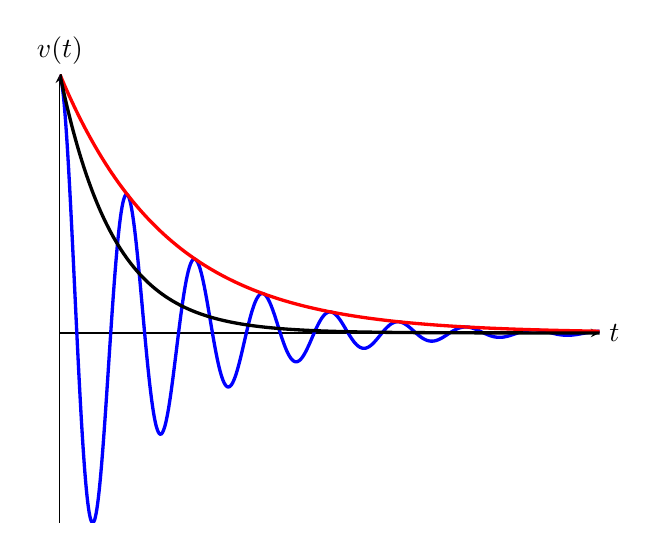
\begin{tikzpicture}
        \begin{axis}[domain=0:5,samples=501,axis lines=center,
        xtick=\empty,ytick=\empty,
        xlabel={$t$},xlabel style={anchor=west},
        ylabel={$v(t)$},ylabel style={anchor=south}]
        \addplot[color=blue,no marks,very thick,smooth] {(exp(-x)*cos(10*deg(x)))};
        \addplot[color=red,no marks, very thick, smooth] {(exp(-x))};
        \addplot[color=black, no marks, very thick, smooth] {(exp(-2 * x))};
        \end{axis}
    \end{tikzpicture}
    }

    \end{enumerate}


%     Solve the differential equation. Considering all of these cases.

% 	\sol{The general solution to the trsolient equation of this form is \[V_{out}(t)=K_1e^{\lambda_1 t}+K_2e^{\lambda_2 t}\]
% 	where
% 	\[\lambda_1=-\alpha +\sqrt{\alpha^2-\omega_0^2}  \]
% 	\[\lambda_2=-\alpha -\sqrt{\alpha^2-\omega_0^2}\]
% 	In this case,
% 	\[\alpha=\frac{1}{2R_sC}\]
% 	\[\omega_0=\frac{1}{\sqrt{LC}}\]
% 	Now to find the constants $K_1$ and $K_2$, we use the initial conditions for $v_{out}(0)$ and $\frac{dv_{out}(0)}{dt}$ and set the general solution to these values:
% 	\begin{align*}
% 		\frac{dv_{out}(0)}{dt}=\frac{V_s}{R_sC}&=K_1\lambda_1+K_2\lambda_2 \\
% 	v_{out}(0)=0&=K_1+K_2 \\
% 	\frac{V_s}{R_sC}&=-K_2\lambda_1+K_2\lambda_2 \\
% 	K_2&=\frac{V_s}{R_sC(\lambda_2-\lambda_1)} \\
% 	K_1&=-\frac{V_s}{R_sC(\lambda_2-\lambda_1)}
% 	\end{align*}
% 	Finally, plugging back into the general solution:
% 	\[V_{out}(t)=-\frac{V_s}{R_sC(\lambda_2-\lambda_1)}e^{\lambda_1 t}+\frac{V_s}{R_sC(\lambda_2-\lambda_1)}e^{\lambda_2 t}\]

% 	For the $\lambda_1=\lambda_2$, which happens in a critically damped system, the general solution is:
% \[V_c=K_1e^{\lambda t}+tK_2e^{\lambda t}\]
% and
% \[\frac{dV_c}{dt}=K_1\lambda e^{\lambda t}+K_2e^{\lambda_t}+t K_2 \lambda e^{\lambda t}\]
% so when plugging our initial conditions into these equations
% \begin{align*}
% V_{out}(0)&=0=K_1 \\
% \frac{dV_c (0)}{dt}&=\frac{V_s}{R_sC}=K_1\lambda+K_2 \\
% K_2&= \frac{V_s}{R_sC} \\
% K_1&=0 \\
% K_2&=\frac{V_s}{R_sC}
% \end{align*}




\end{qunlist}

\end{document}
